\documentclass[a4paper,12pt]{article}
\usepackage[utf8]{inputenc} % Для поддержки UTF-8
\usepackage[T2A]{fontenc}   % Кириллический шрифт
\usepackage[russian]{babel} % Русский язык

\usepackage{amsmath}
\usepackage{graphicx}
\usepackage{geometry}
\geometry{left=2cm,right=1.5cm,top=2cm,bottom=2cm}

\usepackage{graphicx}  % Пакет для работы с изображениями
\usepackage{caption}   % Пакет для настройки подписей к изображениям

% Изменяем текст "Рис." на "Рисунок"
\addto\captionsrussian{\renewcommand{\figurename}{Рисунок}}
% Настраиваем разделитель с ":" на " -"
\captionsetup[figure]{labelsep=endash} % Используем длинное тире для разделителя

\usepackage{fancyhdr}  % Пакет для работы с колонтитулами
\pagestyle{fancy}      % Включаем "продвинутый" стиль страниц
\fancyhf{}             % Очищаем существующие настройки
\fancyfoot[C]{\thepage} % Устанавливаем номер страницы по центру нижней части
\renewcommand{\headrulewidth}{0pt} % Убираем линию в верхнем колонтитуле
\renewcommand{\footrulewidth}{0pt} % Убираем линию в нижнем колонтитуле

\begin{document}

\begin{center}
    \textbf{\Large Одномерные методы оптимизации второго порядка} \\[1cm] % Заголовок жирным
\end{center}

\textbf{Задача оптимизации} — это задача при решении которой требуется добиться минимума (реже максимума) некоторого критерия при заданных ограничениях. \cite{maslennicov}
\begin{figure}[h]  % Начало окружения для вставки изображения
    \centering     % Центрирование изображения
    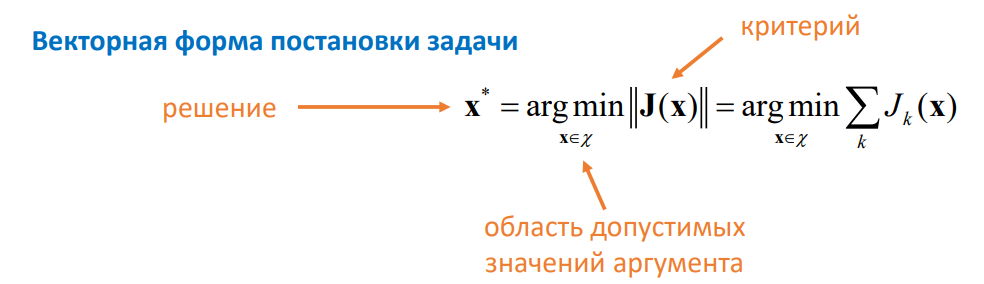
\includegraphics[width=0.8\textwidth]{task.png}  % Вставка изображения, изменяя его ширину
    \caption{Векторная форма постановки задачи}  % Добавление подписи
    \label{fig:img-task}  % Установка метки для ссылки на изображение
\end{figure}

\textbf{Методы второго порядка} — это методы поиска экстремума функций нескольких переменных, где шаг поиска минимума определяется матрицей Гессе:
\begin{equation}
    \mathbf{x}_k = \mathbf{x}_{k-1} + \mathbf{H}^{-1}(\mathbf{x}_{k-1}) \nabla f(\mathbf{x}_{k-1}),
\end{equation}
где \( \mathbf{H}(\mathbf{x}_k) \) — матрица Гессе:
\[
    \mathbf{H}(\mathbf{x}_k) = 
    \begin{bmatrix}
        \frac{\partial^2 f(\mathbf{x})}{\partial x_1^2} & \cdots & \frac{\partial^2 f(\mathbf{x})}{\partial x_1 \partial x_n} \\
        \vdots & \ddots & \vdots \\
        \frac{\partial^2 f(\mathbf{x})}{\partial x_n \partial x_1} & \cdots & \frac{\partial^2 f(\mathbf{x})}{\partial x_n^2}
    \end{bmatrix}_{\mathbf{x}_k}.
\]

\vspace{0.3cm}

Основным таким методом является \textbf{метод Ньютона—Рафсона}:
\begin{equation}
    \mathbf{x}_{k+1} = \mathbf{x}_k + \lambda_k \mathbf{H}^{-1}(\mathbf{x}_k) \nabla f(\mathbf{x}_k),
\end{equation}
где \( \lambda_k \) находится из решения оптимизационной задачи:
\begin{equation}
    \lambda_k = \arg \min_{\lambda_k} f\left( \mathbf{x}_k + \lambda_k \mathbf{H}^{-1}(\mathbf{x}_k) \nabla f(\mathbf{x}_k) \right).
\end{equation}

\vspace{0.3cm}

\textbf{Проблемы применения методов второго порядка:}
\begin{enumerate}
    \item вычисление матрицы Гессе (большой объем вычислений, особенно численных);
    \item вычисление обратной матрицы Гессе (большой объем вычислений, потенциальная неустойчивость). \cite{maslennicov}
\end{enumerate}

\renewcommand{\refname}{Список использованных источников}
\begin{thebibliography}{9}

\bibitem{grebennikova}
И.В. Гребенникова. \textit{Методы оптимизации: учебное пособие}. Екатеринбург: УрФУ, 2017. — 148 с. ISBN 978-5-7996-2090-5.

\bibitem{maslennicov}
Масленников, А.Л. \textit{Методы вычислений: Численные методы поиска экстремумов функций}. Презентация, МГТУ им. Н.Э. Баумана, 2023.

\end{thebibliography}

\begin{flushright}
    О.Н. Талышева ИУ7-55Б
\end{flushright}

\end{document}
